\SourceLeaf{189}2) fährt er fort: »wonach jede im Weltraum von einem Fixstern zum andern, die $90^{0}$ von einander entfernt sind, gezogene Linie eine Tangente der Erdkugel sein würde«. Hierbei ist die Entfernung der Fixsterne verglichen mit der Constante als unermesslich gross betrachtet, aber demungeachtet hat das um $90^{0}$ von einander entfernt sein dann nur einen bestimmten Sinn, in so fern es auf einen bestimmten Scheitelpunkt des Winkels bezogen wird, z.\,B. den Mittelpunkt der Erde, was ohne Zweifel auch Hr. Prof. \textsc{Sch.} tacite vorausgesetzt hat.

3) hat ohne Zweifel diess Hr. Prof. \textsc{Sch.} bloss Beispielshalber als Erläuterung gesagt, denn obgleich ich mir recht gut die Unrichtigkeit der Euklidischen Geometrie denken kann, so müsste doch nach unsern astronomischen Erfahrungen die besagte Constante unermesslich viel grösser sein, als der Erdradius.

Ich vermuthe, dass Hr. \textsc{Sch.} mit allem diesen einverstanden sein wird, was mich bei dem gänzlichen Zusammentreffen seiner Ansicht mit der meinigen sehr freuen wird. Ich bemerke nur noch, dass ich die Astralgeometrie so weit ausgebildet habe, dass ich alle Aufgaben vollständig auflösen kann, sobald die Constante $= C$ gegeben wird. Der Defect der Winkelsumme im ebenen Dreieck gegen $180^{0}$ ist z.\,B. nicht bloss desto grösser, je grösser der Flächeninhalt ist, sondern ihm genau proportional, so dass der Flächeninhalt eine Grenze hat, die er nie erreichen kann, und welche Grenze selbst dem Inhalt der zwischen drei sich asymptotisch berührenden geraden Linien enthaltenen Fläche gleich ist, die Formel für diese Grenze ist
\begin{center}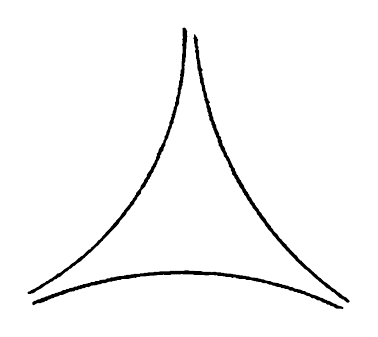
\begin{tikzpicture}[x=0.00650530cm,y=-0.00650530cm]
\fill[even odd rule] (31,546) -- (31,549) -- (33,551) -- (34,551) -- (41,547) -- (48,547) -- (49,546) -- (54,545) -- (56,543) -- (59,543) -- (63,540) -- (65,540) -- (68,538) -- (73,537) -- (75,535) -- (81,534) -- (86,531) -- (90,531) -- (104,525) -- (113,524) -- (115,522) -- (119,522) -- (122,520) -- (125,520) -- (129,518) -- (133,518) -- (137,515) -- (141,516) -- (146,513) -- (157,512) -- (158,511) -- (164,510) -- (168,508) -- (174,508) -- (181,505) -- (187,505) -- (188,504) -- (196,503) -- (197,502) -- (203,502) -- (206,500) -- (220,500) -- (221,499) -- (224,499) -- (225,498) -- (228,498) -- (229,497) -- (233,498) -- (236,496) -- (241,496) -- (242,495) -- (253,495) -- (254,494) -- (274,493) -- (275,492) -- (286,492) -- (287,491) -- (289,492) -- (301,492) -- (302,491) -- (321,491) -- (322,490) -- (324,490) -- (325,491) -- (346,491) -- (347,492) -- (367,492) -- (368,493) -- (376,493) -- (377,492) -- (386,492) -- (387,493) -- (389,493) -- (391,492) -- (394,494) -- (403,494) -- (404,495) -- (408,495) -- (409,496) -- (418,496) -- (422,498) -- (424,497) -- (428,497) -- (430,499) -- (434,499) -- (435,500) -- (447,500) -- (450,502) -- (459,502) -- (460,503) -- (463,503) -- (464,504) -- (468,504) -- (469,505) -- (478,506) -- (482,508) -- (488,508) -- (494,511) -- (498,511) -- (501,513) -- (504,513) -- (508,515) -- (516,516) -- (518,518) -- (523,518) -- (524,519) -- (531,520) -- (535,523) -- (540,523) -- (543,525) -- (547,525) -- (550,527) -- (553,527) -- (557,529) -- (560,529) -- (568,533) -- (573,534) -- (578,538) -- (581,537) -- (589,542) -- (593,542) -- (599,546) -- (604,547) -- (607,550) -- (611,550) -- (613,552) -- (620,554) -- (622,556) -- (626,558) -- (635,558) -- (637,559) -- (639,557) -- (639,556) -- (636,554) -- (628,552) -- (624,549) -- (620,548) -- (611,543) -- (608,543) -- (606,541) -- (604,541) -- (597,537) -- (595,537) -- (587,533) -- (576,530) -- (573,528) -- (566,526) -- (564,524) -- (561,524) -- (555,521) -- (544,519) -- (539,516) -- (535,516) -- (530,513) -- (526,513) -- (525,512) -- (519,511) -- (518,510) -- (515,510) -- (511,508) -- (502,507) -- (495,504) -- (491,504) -- (490,503) -- (487,503) -- (483,501) -- (479,501) -- (478,500) -- (472,499) -- (471,498) -- (458,497) -- (454,495) -- (449,495) -- (448,494) -- (443,494) -- (442,493) -- (436,493) -- (435,492) -- (429,492) -- (428,491) -- (423,491) -- (422,490) -- (406,489) -- (405,488) -- (400,488) -- (399,487) -- (391,487) -- (390,486) -- (384,486) -- (383,487) -- (381,487) -- (380,486) -- (364,486) -- (363,485) -- (337,484) -- (336,483) -- (329,483) -- (328,484) -- (301,484) -- (300,485) -- (280,485) -- (279,486) -- (269,486) -- (268,487) -- (257,487) -- (256,488) -- (250,488) -- (249,489) -- (242,489) -- (241,490) -- (230,490) -- (229,491) -- (224,491) -- (223,492) -- (215,492) -- (214,493) -- (211,493) -- (210,494) -- (196,495) -- (195,496) -- (192,496) -- (191,497) -- (185,497) -- (182,499) -- (177,499) -- (175,501) -- (164,502) -- (161,504) -- (155,504) -- (152,506) -- (147,506) -- (143,508) -- (140,508) -- (139,509) -- (136,509) -- (135,510) -- (131,510) -- (128,512) -- (125,512) -- (124,513) -- (121,513) -- (118,515) -- (114,515) -- (111,517) -- (104,518) -- (101,520) -- (98,520) -- (95,522) -- (91,522) -- (86,525) -- (84,525) -- (80,527) -- (77,527) -- (74,529) -- (69,530) -- (66,532) -- (63,532) -- (61,534) -- (58,534) -- (55,536) -- (50,537) -- (45,540) -- (42,540) -- (37,543) -- (35,543) -- cycle
(347,22) -- (347,28) -- (346,29) -- (346,31) -- (347,32) -- (347,39) -- (349,41) -- (348,43) -- (348,45) -- (350,49) -- (350,53) -- (349,54) -- (349,56) -- (351,60) -- (351,69) -- (352,70) -- (352,73) -- (353,74) -- (354,91) -- (356,94) -- (356,99) -- (357,100) -- (357,103) -- (358,104) -- (358,109) -- (359,110) -- (359,116) -- (362,122) -- (362,125) -- (363,126) -- (363,132) -- (365,135) -- (366,143) -- (368,147) -- (367,150) -- (369,153) -- (369,155) -- (371,159) -- (371,164) -- (373,168) -- (373,173) -- (375,175) -- (375,177) -- (376,178) -- (375,181) -- (377,183) -- (377,189) -- (381,194) -- (381,198) -- (383,201) -- (383,204) -- (385,206) -- (385,209) -- (387,212) -- (387,214) -- (390,220) -- (390,222) -- (393,226) -- (393,231) -- (395,235) -- (395,239) -- (398,242) -- (399,246) -- (405,256) -- (405,259) -- (406,261) -- (409,264) -- (411,269) -- (413,271) -- (413,273) -- (415,277) -- (415,280) -- (419,284) -- (419,288) -- (422,292) -- (421,295) -- (426,300) -- (426,302) -- (430,307) -- (430,310) -- (434,315) -- (436,320) -- (441,326) -- (442,330) -- (445,333) -- (445,335) -- (448,338) -- (452,346) -- (455,349) -- (456,352) -- (461,358) -- (461,360) -- (469,369) -- (470,373) -- (474,377) -- (475,380) -- (485,392) -- (486,395) -- (491,401) -- (491,402) -- (498,409) -- (501,414) -- (507,420) -- (507,421) -- (518,433) -- (518,434) -- (526,442) -- (526,443) -- (532,448) -- (532,449) -- (545,462) -- (545,463) -- (555,472) -- (556,474) -- (557,474) -- (563,480) -- (568,483) -- (587,501) -- (588,501) -- (593,506) -- (594,506) -- (598,510) -- (599,510) -- (606,517) -- (612,520) -- (613,522) -- (614,522) -- (617,525) -- (619,525) -- (632,537) -- (635,538) -- (637,540) -- (639,540) -- (646,546) -- (649,546) -- (651,544) -- (651,543) -- (644,536) -- (639,534) -- (631,527) -- (628,526) -- (623,521) -- (615,516) -- (610,511) -- (609,511) -- (606,508) -- (601,505) -- (595,499) -- (590,496) -- (586,491) -- (585,491) -- (571,478) -- (570,478) -- (558,466) -- (557,464) -- (555,464) -- (551,460) -- (548,455) -- (546,453) -- (545,453) -- (528,435) -- (528,433) -- (526,432) -- (519,425) -- (519,424) -- (514,420) -- (510,413) -- (503,407) -- (501,403) -- (498,400) -- (497,397) -- (490,389) -- (487,383) -- (480,375) -- (479,372) -- (474,367) -- (474,365) -- (468,358) -- (468,357) -- (466,355) -- (466,353) -- (462,349) -- (458,341) -- (455,338) -- (455,336) -- (453,334) -- (452,331) -- (449,328) -- (448,325) -- (446,323) -- (444,317) -- (439,310) -- (439,308) -- (436,305) -- (435,302) -- (433,300) -- (433,298) -- (430,295) -- (430,293) -- (427,288) -- (427,285) -- (424,282) -- (415,262) -- (411,257) -- (411,254) -- (408,249) -- (408,246) -- (406,242) -- (403,239) -- (403,236) -- (402,235) -- (402,230) -- (399,226) -- (400,223) -- (396,220) -- (396,216) -- (391,206) -- (390,199) -- (388,197) -- (388,195) -- (385,189) -- (385,185) -- (383,182) -- (382,175) -- (380,172) -- (380,166) -- (378,164) -- (378,162) -- (376,159) -- (376,157) -- (378,155) -- (378,154) -- (375,151) -- (375,149) -- (373,147) -- (372,138) -- (369,131) -- (369,127) -- (368,126) -- (368,122) -- (367,121) -- (367,117) -- (366,116) -- (366,108) -- (364,106) -- (363,98) -- (362,97) -- (362,94) -- (364,92) -- (364,91) -- (361,88) -- (361,86) -- (360,85) -- (359,73) -- (358,72) -- (358,69) -- (357,68) -- (357,54) -- (355,51) -- (356,47) -- (354,44) -- (354,35) -- (355,34) -- (355,32) -- (353,30) -- (353,28) -- (351,26) -- (349,22) -- cycle
(329,9) -- (327,9) -- (324,11) -- (325,13) -- (325,26) -- (326,28) -- (324,32) -- (325,34) -- (325,40) -- (324,41) -- (324,44) -- (325,45) -- (325,59) -- (324,60) -- (324,70) -- (323,71) -- (324,73) -- (323,75) -- (323,90) -- (321,92) -- (321,99) -- (320,100) -- (320,103) -- (321,105) -- (320,106) -- (320,111) -- (318,113) -- (318,120) -- (317,121) -- (317,125) -- (315,128) -- (316,134) -- (315,135) -- (315,139) -- (312,146) -- (312,153) -- (310,155) -- (310,161) -- (307,166) -- (307,170) -- (305,174) -- (305,177) -- (303,179) -- (304,182) -- (302,185) -- (302,188) -- (299,194) -- (299,200) -- (297,202) -- (296,207) -- (293,213) -- (293,216) -- (291,220) -- (289,222) -- (290,225) -- (289,226) -- (289,228) -- (287,230) -- (287,233) -- (284,237) -- (282,242) -- (280,244) -- (278,248) -- (277,253) -- (275,255) -- (274,255) -- (275,259) -- (273,262) -- (273,265) -- (270,270) -- (270,272) -- (267,276) -- (266,279) -- (264,281) -- (263,285) -- (255,296) -- (255,300) -- (250,306) -- (249,310) -- (243,318) -- (242,323) -- (234,332) -- (234,335) -- (231,338) -- (231,340) -- (227,344) -- (227,346) -- (222,351) -- (221,354) -- (210,367) -- (210,368) -- (207,371) -- (202,379) -- (195,386) -- (195,387) -- (189,393) -- (189,394) -- (184,399) -- (184,400) -- (174,410) -- (174,411) -- (167,418) -- (167,419) -- (162,424) -- (161,424) -- (158,427) -- (158,428) -- (149,437) -- (148,437) -- (146,439) -- (146,440) -- (144,442) -- (141,443) -- (137,447) -- (136,447) -- (135,449) -- (129,455) -- (126,456) -- (123,459) -- (122,459) -- (115,466) -- (107,471) -- (102,476) -- (94,481) -- (87,487) -- (83,489) -- (81,489) -- (75,495) -- (74,495) -- (69,499) -- (66,500) -- (61,504) -- (59,504) -- (56,507) -- (48,511) -- (42,516) -- (40,516) -- (38,518) -- (29,522) -- (27,524) -- (23,525) -- (22,526) -- (22,528) -- (23,529) -- (28,529) -- (29,528) -- (32,528) -- (36,526) -- (39,523) -- (49,518) -- (58,511) -- (61,510) -- (68,505) -- (70,505) -- (74,501) -- (78,500) -- (81,497) -- (85,496) -- (96,486) -- (99,485) -- (104,480) -- (106,480) -- (111,475) -- (114,474) -- (118,470) -- (126,465) -- (132,459) -- (133,459) -- (136,455) -- (137,455) -- (143,449) -- (144,449) -- (157,436) -- (158,436) -- (167,426) -- (169,425) -- (169,424) -- (199,393) -- (203,386) -- (214,374) -- (216,369) -- (222,363) -- (224,359) -- (230,353) -- (231,349) -- (236,343) -- (236,341) -- (243,333) -- (244,327) -- (252,319) -- (253,315) -- (257,309) -- (257,307) -- (261,303) -- (261,301) -- (263,299) -- (264,295) -- (268,290) -- (268,288) -- (271,282) -- (273,280) -- (273,278) -- (275,275) -- (276,270) -- (279,267) -- (279,265) -- (281,263) -- (281,258) -- (283,256) -- (283,253) -- (287,249) -- (288,243) -- (291,239) -- (291,234) -- (292,233) -- (292,231) -- (297,223) -- (297,220) -- (299,217) -- (299,214) -- (300,213) -- (301,208) -- (303,205) -- (304,199) -- (307,195) -- (307,190) -- (310,183) -- (310,180) -- (311,179) -- (311,176) -- (312,175) -- (314,164) -- (318,157) -- (318,148) -- (319,147) -- (319,143) -- (320,142) -- (320,139) -- (321,138) -- (321,131) -- (323,128) -- (323,124) -- (325,121) -- (324,118) -- (326,115) -- (325,111) -- (326,110) -- (326,105) -- (327,104) -- (327,99) -- (328,98) -- (328,91) -- (329,90) -- (328,88) -- (328,84) -- (329,83) -- (328,79) -- (330,75) -- (330,68) -- (331,67) -- (331,51) -- (332,50) -- (332,38) -- (333,37) -- (333,28) -- (334,27) -- (334,25) -- (333,24) -- (333,18) -- (334,16) -- (332,14) -- (332,12) -- cycle;
\end{tikzpicture}
\end{center}
\[
\text{Limes areae trianguli plani} = \frac{\pi CC}{\{\log\mathrm{hyp}\,(1+\sqrt{2})\}^{2}}.
\]



Auch jedes andere Polygon von einer bestimmten Seitenzahl $= n$ hat in Beziehung auf seinen Flächeninhalt eine bestimmte Grenze, der es so nahe man will kommen, aber sie nie erreichen kann,

\[
= \frac{(n-2)\pi CC}{(\log\mathrm{hyp}\,(1+\sqrt{2}))^{2}}.
\]

Theilen Sie gefälligst diess Hrn. \textsc{Schw.} mit. .\ .\ .\ .\ .\ .

\bigskip
\noindent\hrulefill

